\section{Exploratory Data Analysis}
\label{sec:datAnalisys}

\subsection{Hypothesis}

During the data analysis we stated different hypothesis:

\begin{itemize}

\item \textbf{H1}: Due to UBER incursion in the city, the \textbf{travel distances} of yellow cabs trips increased.

\item \textbf{H2}: Due to UBER incursion in the city, the \textbf{number of trips} of yellow cabs was reduced.

\item \textbf{H3}: The areas of the city where there is \textbf{no public transportation} coverage, especially for hire transportation, correspond to areas with \textbf{low income families}. 

\item \textbf{H4}: Due to UBER incursion in the city, the price of yellow cabs trips have decreased. 

\end{itemize}


\subsection{Data Exploration}

Different plots were created with the aim of understanding the behaviour of the different transportation systems. The following figures show some of the comparisons that were done, and shows the relationship of the plots with the previously mentioned hypothesis.

\subsubsection{General Plots}

Figure \ref{fig:boxTrips} shows the boxplots of the monthly number of trips for the different transportation systems. Figure \ref{fig:a} for Uber's trips, Figure \ref{fig:b} for Yellow cab trips, Figure \ref{fig:c} for Green cab trips, and Figure \ref{fig:d} for MTA trips. The boxplots differentiate the trips between rush hours (orange boxes) and non-rush hours (blue boxes). From the figures, it can be seen that the MTA is busier in rush hours than in non-rush hours. Additionally, it is possible to see that there has been a significant increase of the number of trips taken by Uber from 2015 both in rush and non-rush hours; and a decrease on the number of trips taken by Yellow cabs, especially in rush hours. The latter corresponds to the ideas stated in hypothesis \textbf{H3}.

Figure \ref{fig:boxTripsWeekends} shows the same plot, but separating weekdays (blue boxes) from weekends. In the figure we can also see the previously mentioned behaviour: UBER trips increase and yellow trips tend to decrease.

Additionally, Figure \ref{fig:boxTripsHour} was created to analyze if users prefer to use a specific service at a specific hour. We can see that pick ups are high when people are moving to work, i.e. 7 am (yellow, UBER, and green cabs have a high number of pick ups during that hour). Nevertheless, the highest number of pick ups occur between 6 and 7 pm, the time when many people go home or go out for fun. MTA, on the other hand, shows a different behaviour during the day, with different busy moments.

  
\begin{figure}%
\centering
\subfigure[Uber trips.]{%
\label{fig:a}%
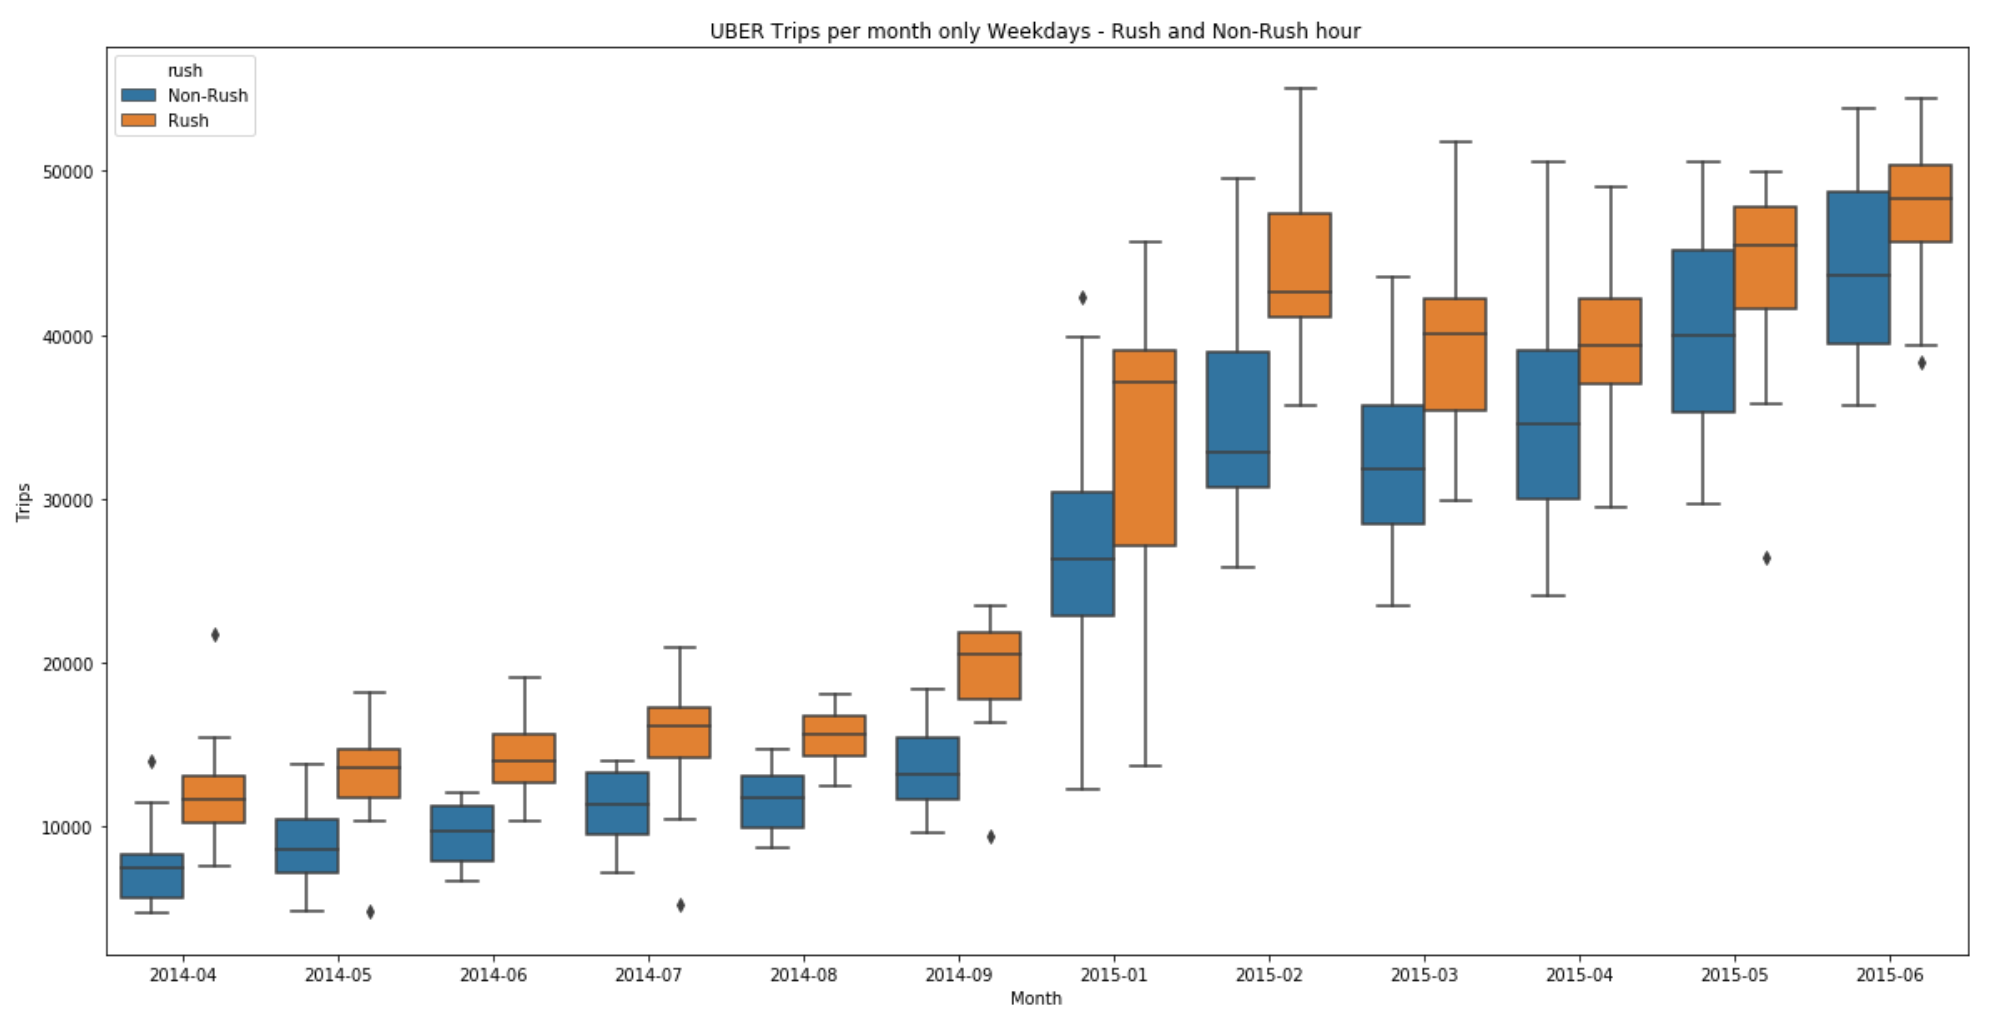
\includegraphics[height=2in, width=3.5in]{UBER_trips_only_weekdays_rush_and_non_rush.png}}%
\qquad
\subfigure[Yellow cab trips]{%
\label{fig:b}%
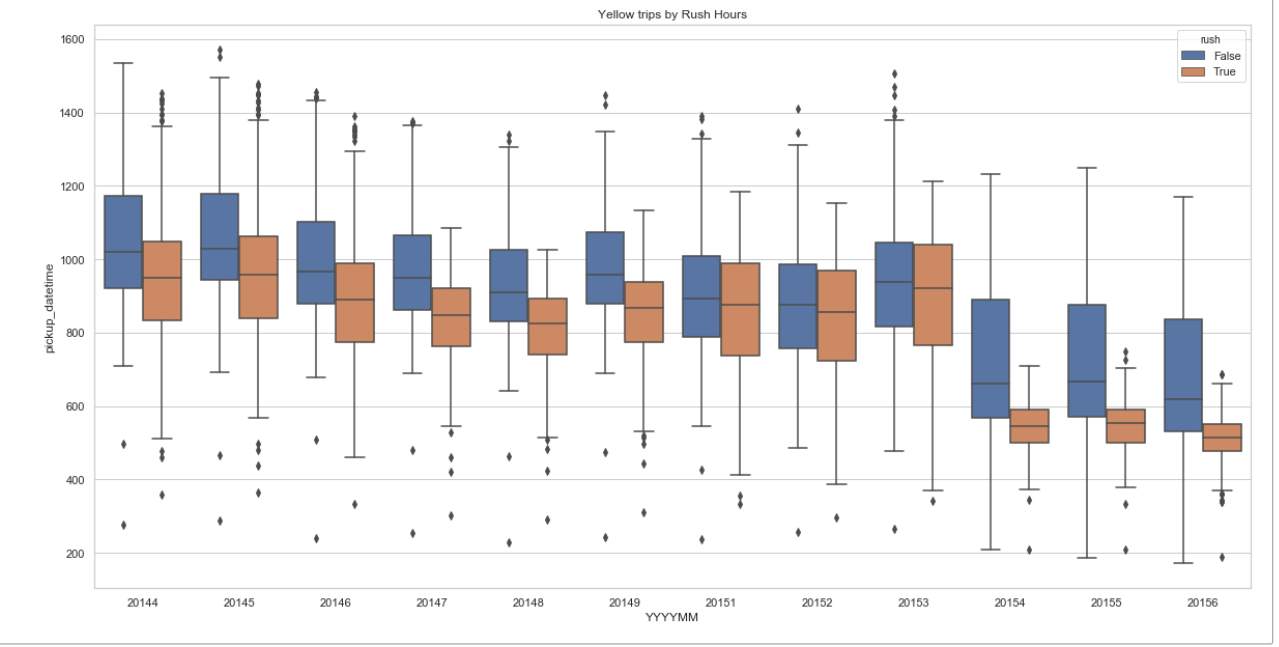
\includegraphics[height=2in, width=3.5in]{yellowTripsRushHours.png}}%
\qquad
\subfigure[Green cab trips]{%
\label{fig:c}%
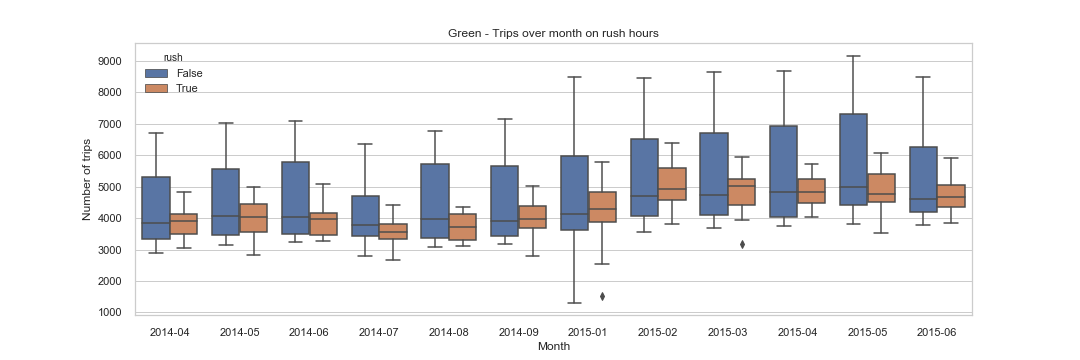
\includegraphics[height=2.4in, width=3.5in]{green_trips_month_rush.png}}%
\qquad
\subfigure[MTA trips]{%
\label{fig:d}%
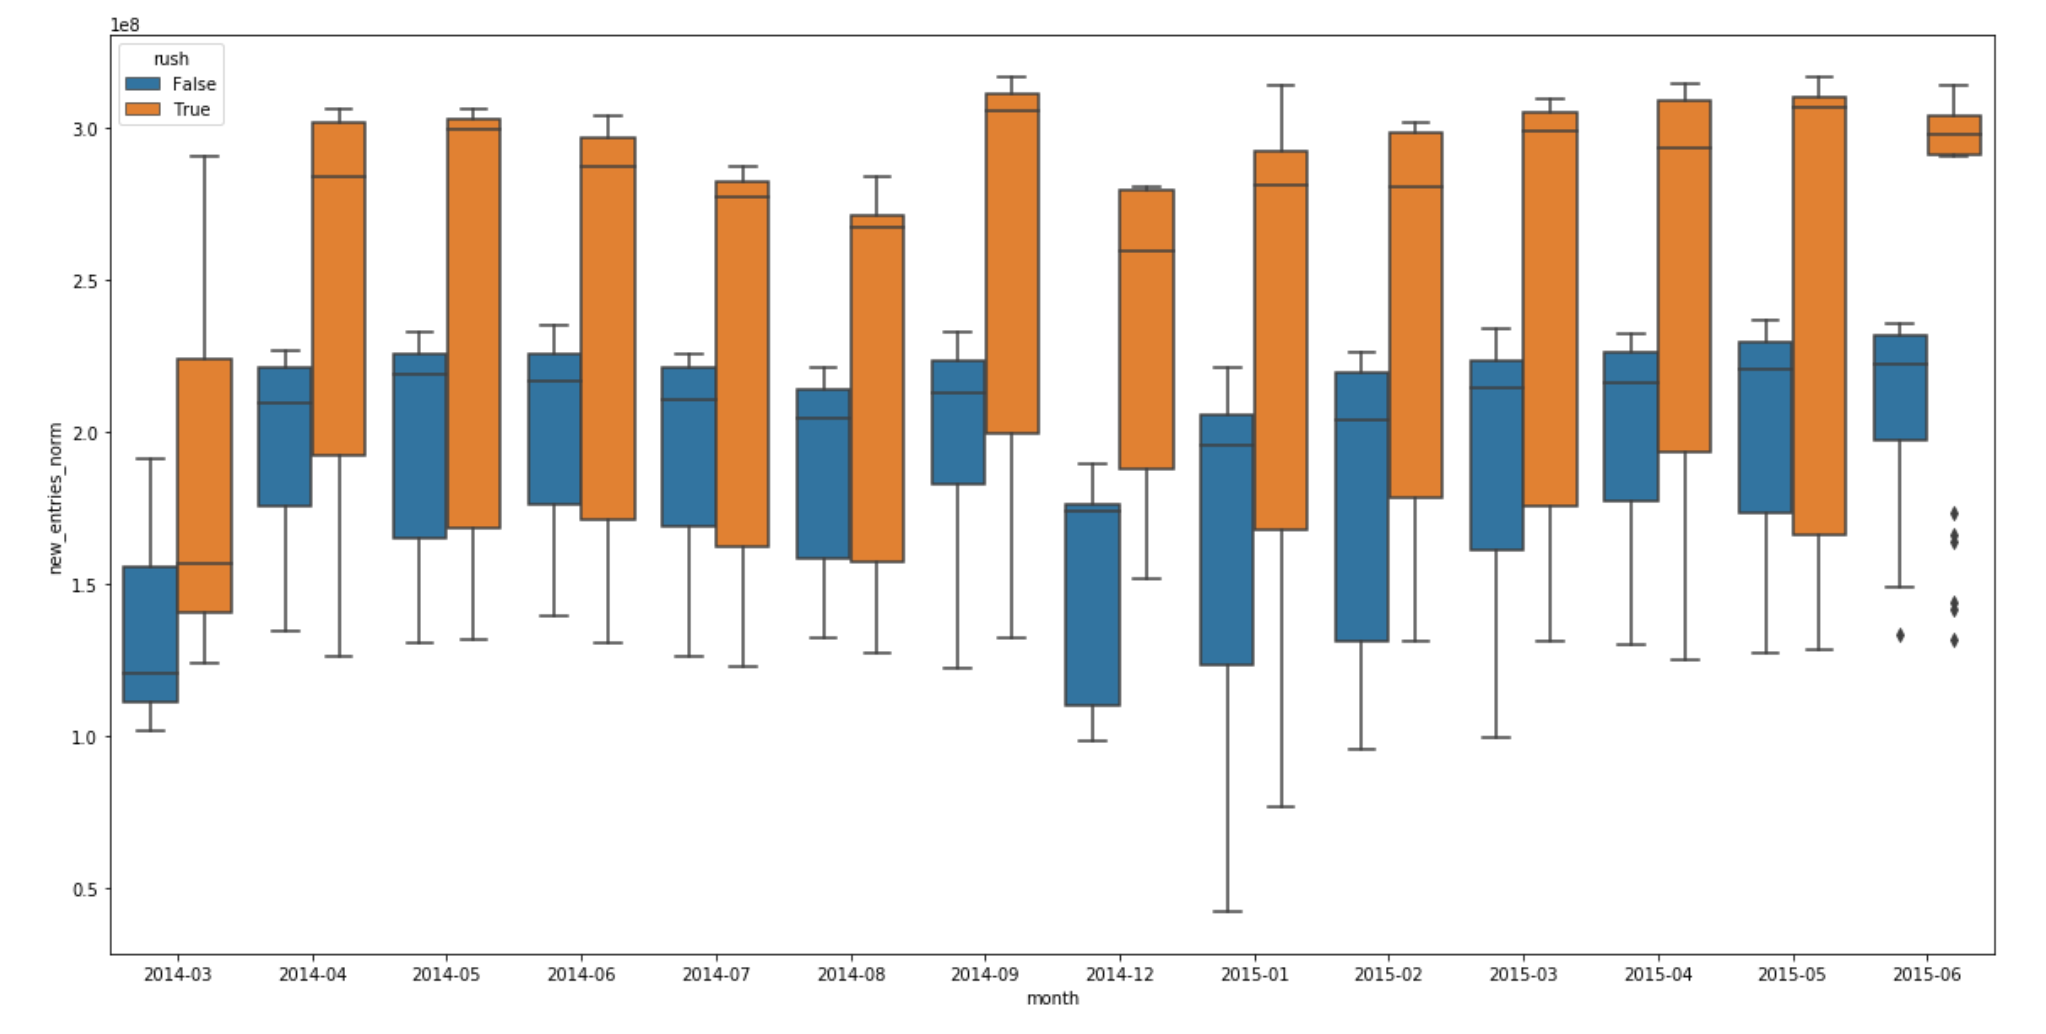
\includegraphics[height=2in, width=3.5in]{mta_new_entries_orange_rush_hour.png}}%
\caption{Has the increase of Uber trips affected the number of trips of Yellow cab, Green cab, and MTA? Orange boxes represent the number of trips in rush hours and blue ones correspond to non-rush hours. }
\label{fig:boxTrips}%
\end{figure}





%Figure \ref{fig:boxDistancesAndPrice} compares the number of trips made by Uber with the monthly average travel distance covered by Yellow cabs. The aim of this comparison was to analyze if the increase of Uber trips affected the average travel distance of   plots, it is possible to see that from 2015, Uber is widely used for long distance trips, in contrast to Yellow cabs. On the other hand, the average travel distance of Yellow cabs experienced an increase in April 2015. 


\begin{figure}%
\centering
\subfigure[Uber trips.]{%
\label{fig:a}%
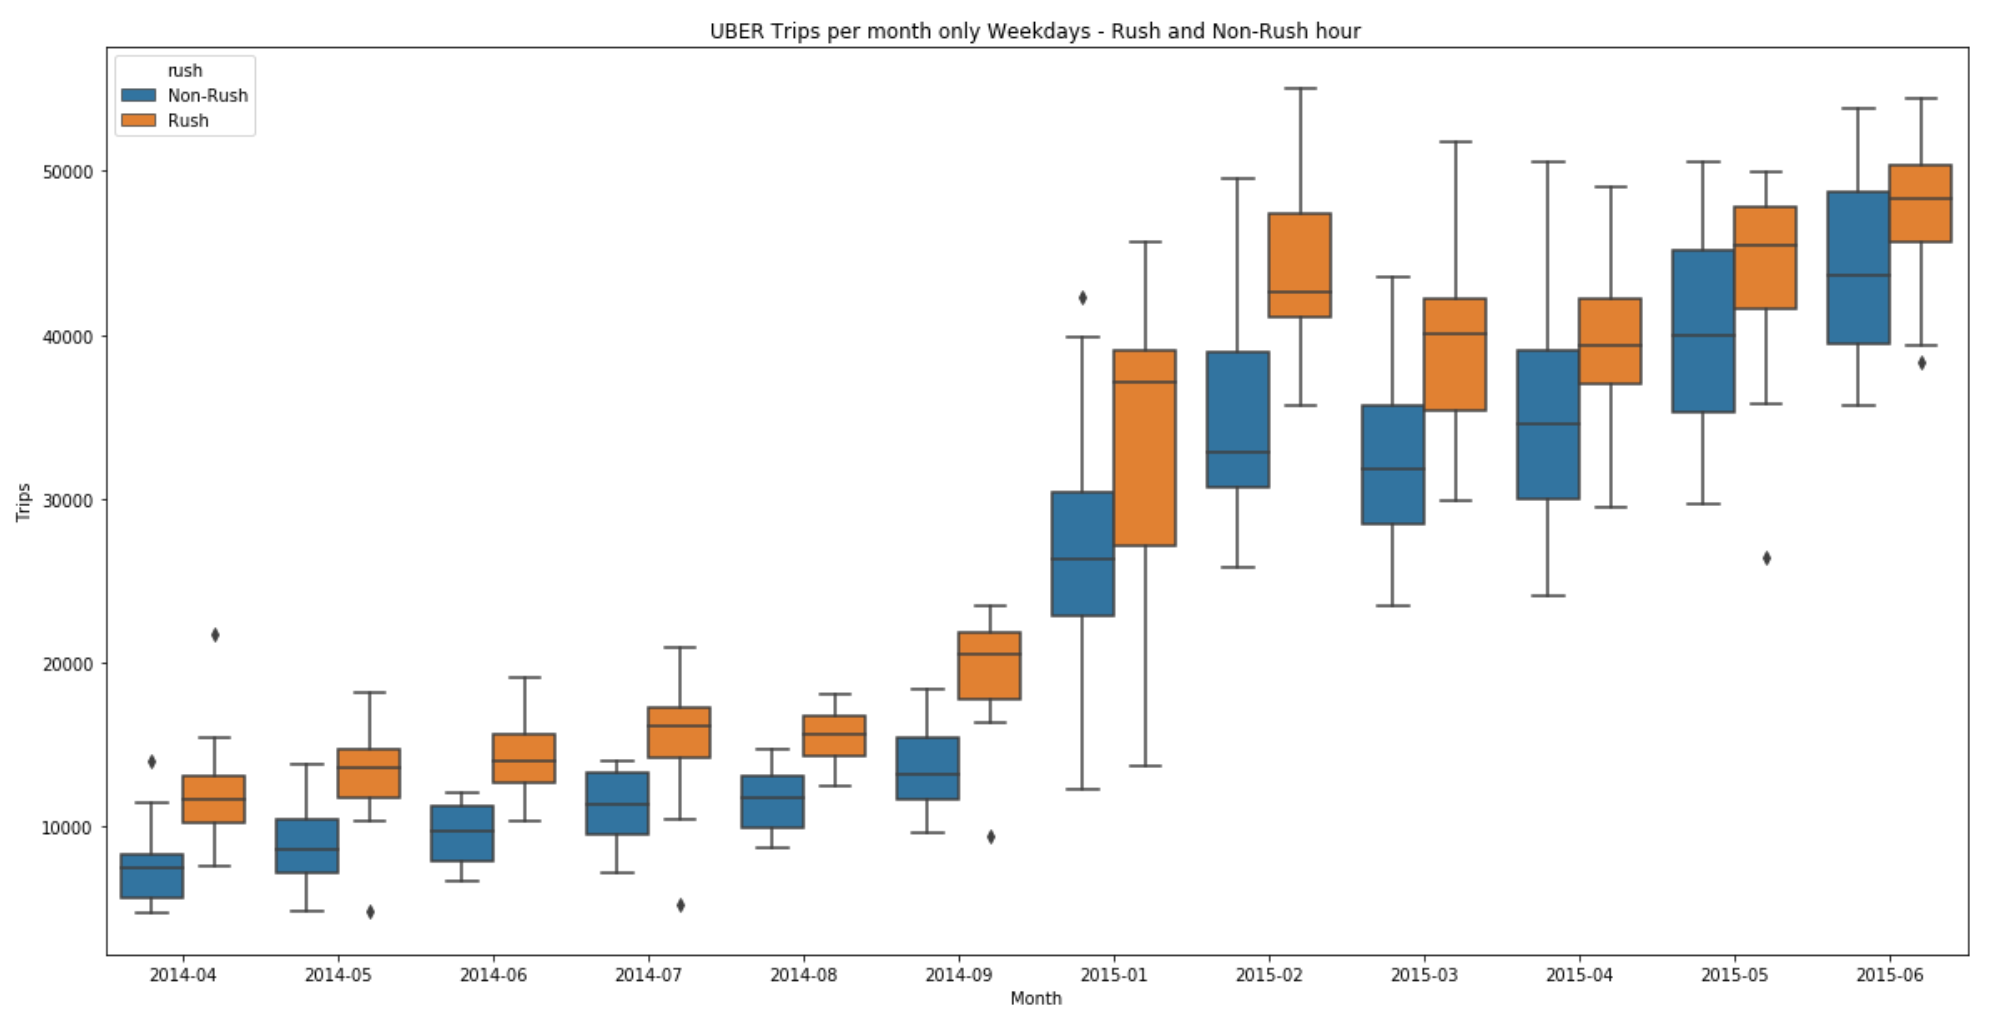
\includegraphics[height=2in, width=3.5in]{UBER_trips_only_weekdays_rush_and_non_rush.png}}%
\qquad
\subfigure[Yellow cab trips]{%
\label{fig:b}%
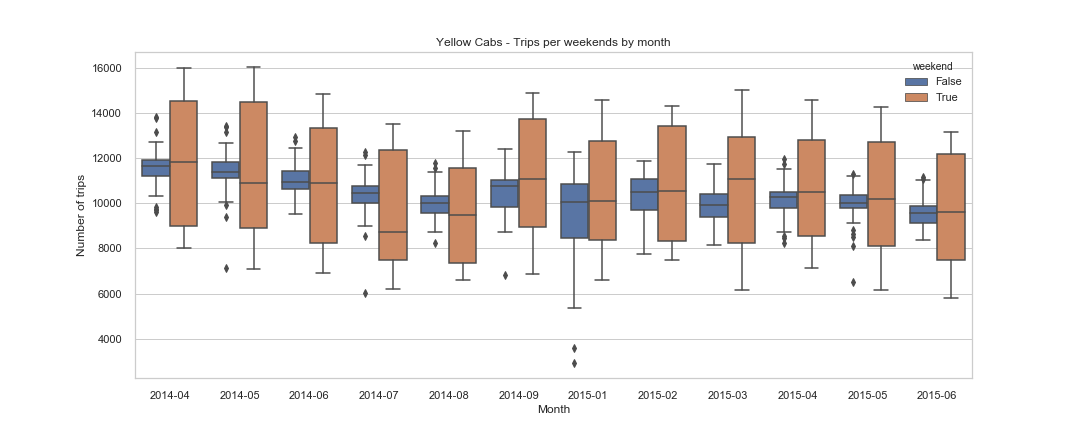
\includegraphics[height=2in, width=3.5in]{yellow_trips_month_weekend.png}}%
\qquad
\subfigure[Green cab trips]{%
\label{fig:c}%
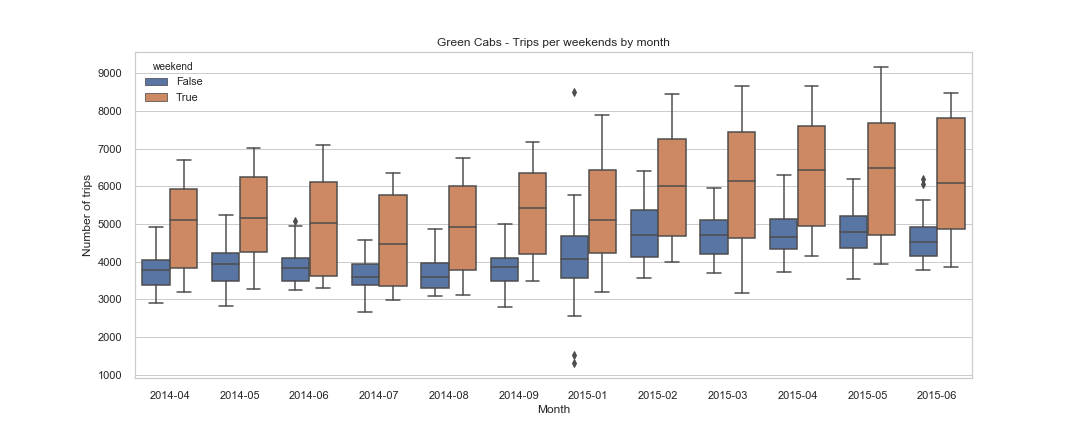
\includegraphics[height=2.4in, width=3.5in]{green_trips_month_weekend.png}}%
\qquad
\subfigure[MTA trips]{%
\label{fig:d}%
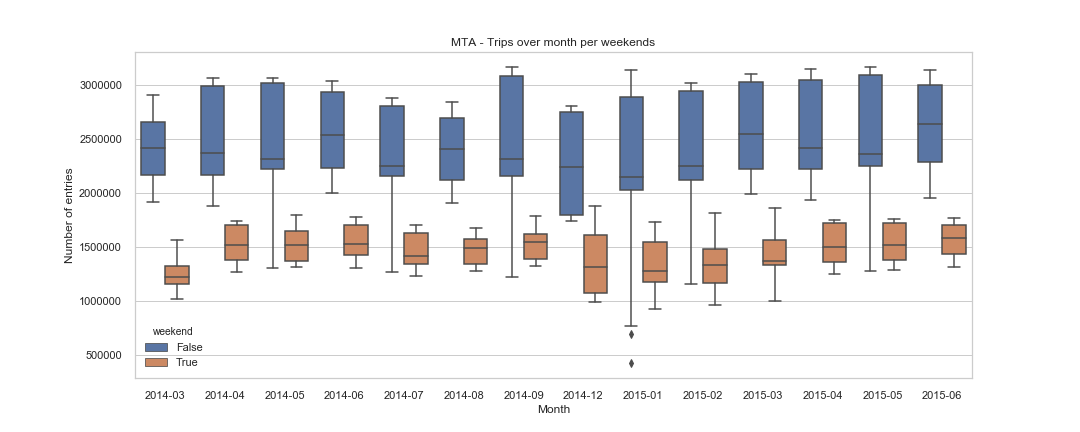
\includegraphics[height=2in, width=3.5in]{mta_entries_month_weekend.png}}%
\caption{Has the increase of Uber trips affected the number of trips of Yellow cab, Green cab, and MTA? Orange boxes represent the number of trips in weekends and blue ones correspond to weekdays. }
\label{fig:boxTripsWeekends}%
\end{figure}






\begin{figure}%
\centering
\subfigure[Uber trips.]{%
\label{fig:a}%
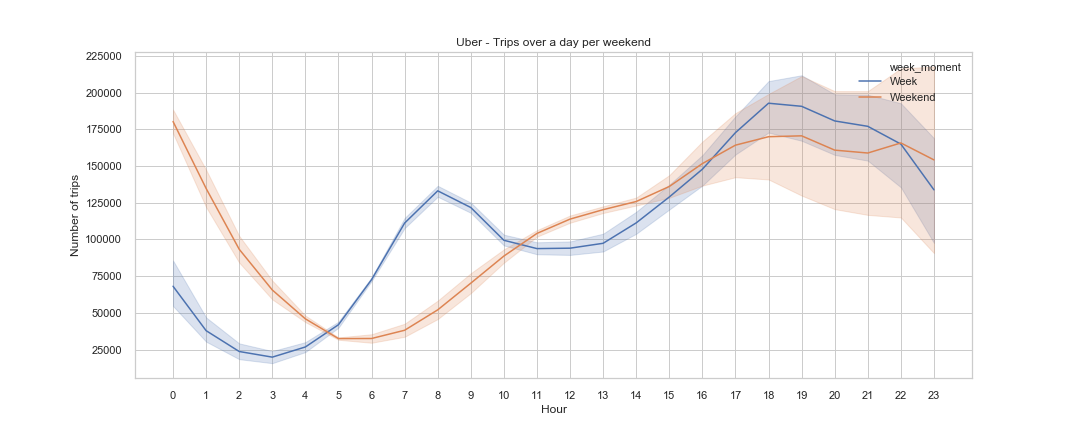
\includegraphics[height=2in, width=3.5in]{uber_trips_hour_week.png}}%
\qquad
\subfigure[Yellow cab trips]{%
\label{fig:b}%
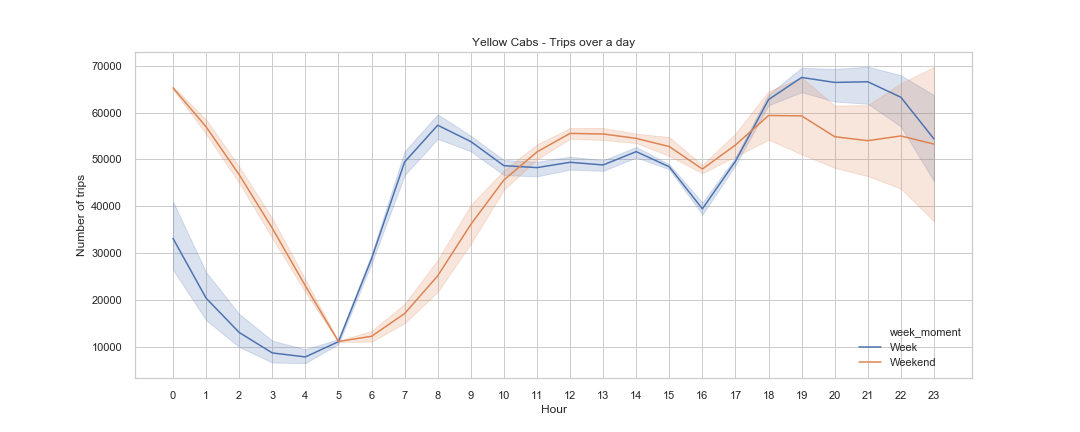
\includegraphics[height=2in, width=3.5in]{yellow_trips_hour_week.png}}%
\qquad
\subfigure[Green cab trips]{%
\label{fig:c}%
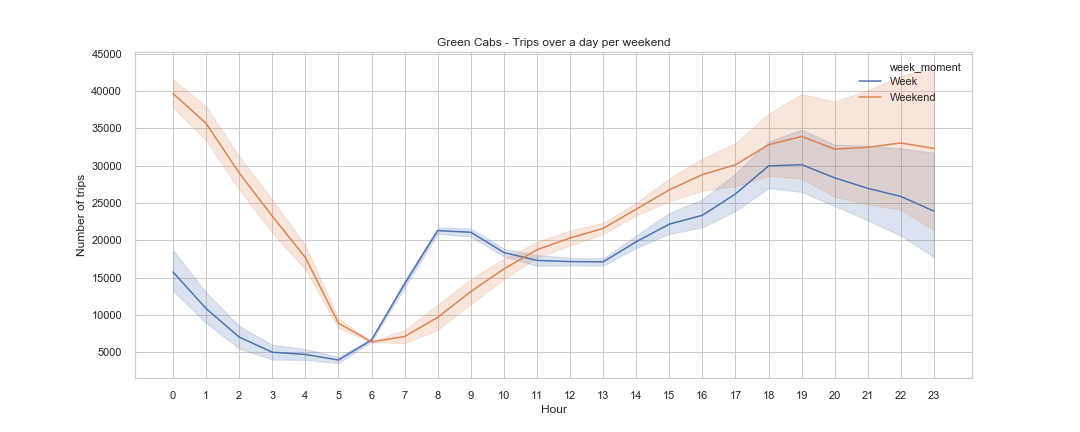
\includegraphics[height=2.4in, width=3.5in]{green_trips_hour_week.png}}%
\qquad
\subfigure[MTA trips]{%
\label{fig:d}%
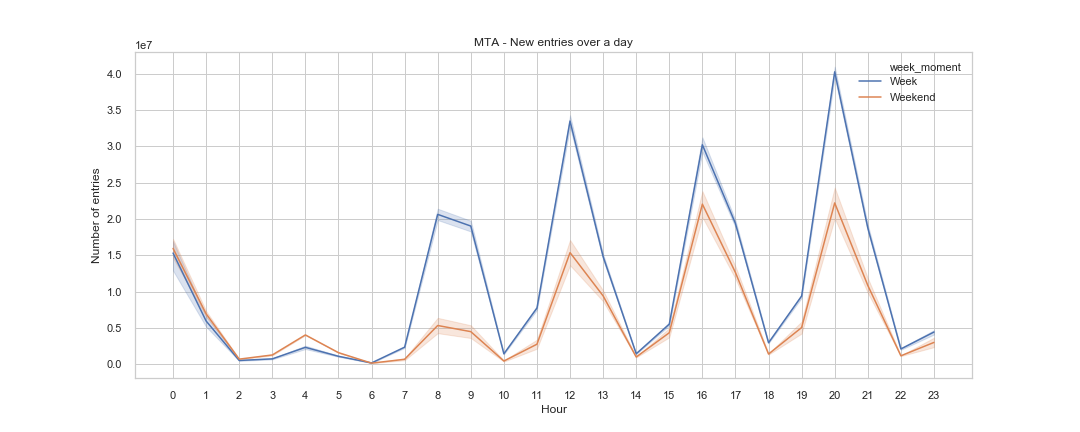
\includegraphics[height=2in, width=3.5in]{mta_entries_hour_week.png}}%
\caption{Behaviour of the number of trips per hour. }
\label{fig:boxTripsWeekends }
\label{fig:boxTripsHour}%
\end{figure}



On the other hand to analyze Hypothesis \textbf{H4}, the plots of Figure \ref{fig:boxDistancesPrice} were created. Figure \ref{fig:boxDistancesPrice_a} and \ref{fig:boxDistancesPrice_c} proof what was mentioned in in Section \ref{intro_background}, the price of a trip by Green cab is cheaper than by Yellow cabs. However, the plots show that the price of Green and Yellow cab trips have not reduced as we thought.


Figures \ref{fig:boxDistancesPrice_b} and \ref{fig:boxDistancesPrice_d} analyze the traveled distances of yellow and green cabs. The plots show that they have not vary significatively, as we stated in Hypothesis \textbf{H1}.


\begin{figure}%
\centering
\subfigure[Yellow cabs. Average price per distance (USD/mile)]{%
\label{fig:boxDistancesPrice_a}%
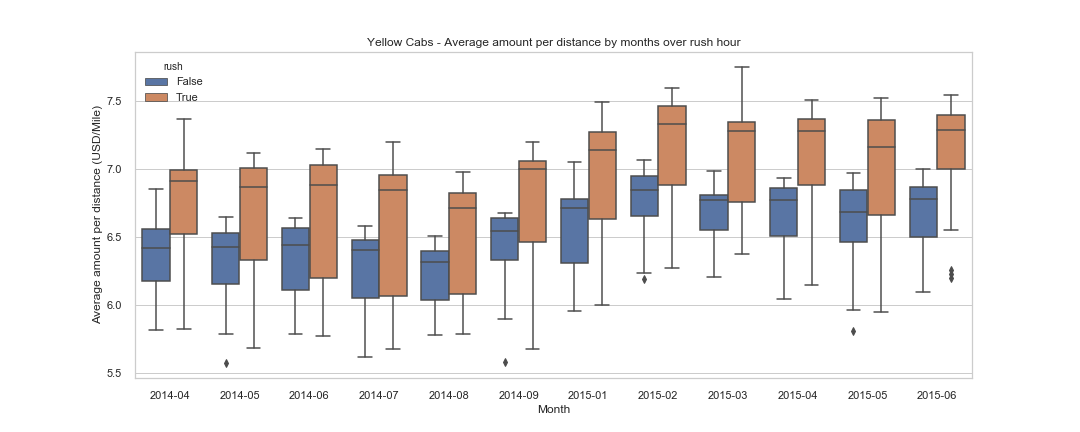
\includegraphics[height=2in, width=3.5in]{yellow_avgamountperdistance_rush_month_boxplot.png}}
\qquad
\subfigure[Yellow cabs. Average distance per month]{%
\label{fig:boxDistancesPrice_b}%
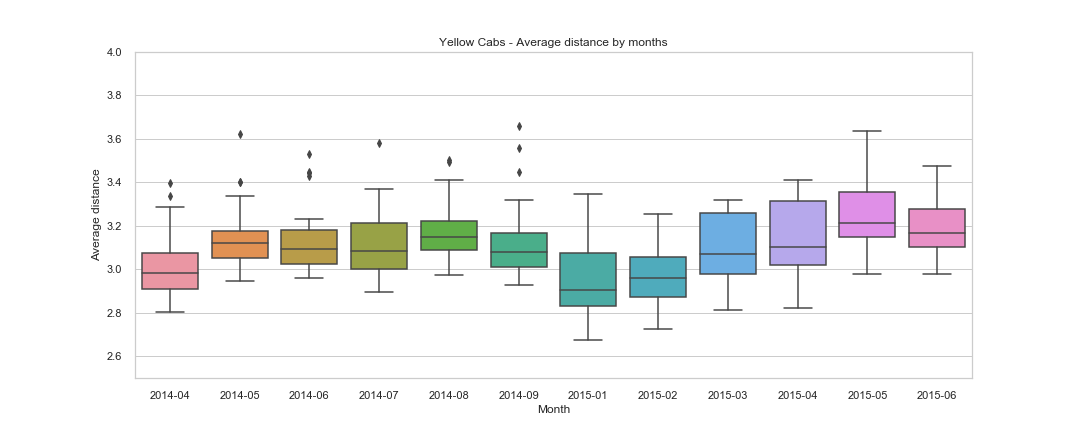
\includegraphics[height=2in, width=3.5in] {yellow_avgdistance_month_boxplot}}
\subfigure[Green cabs. Average price per distance (USD/mile)]{%
\label{fig:boxDistancesPrice_c}%
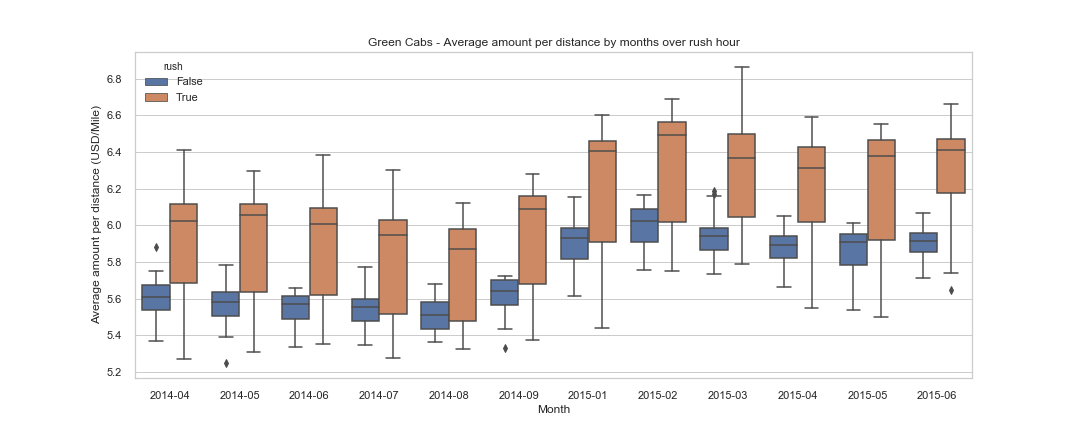
\includegraphics[height=2in, width=3.5in]{green_avgamountperdistance_rush_month_boxplot.png}}
\qquad
\subfigure[Green cabs. Average distance per month]{%
\label{fig:boxDistancesPrice_d}%
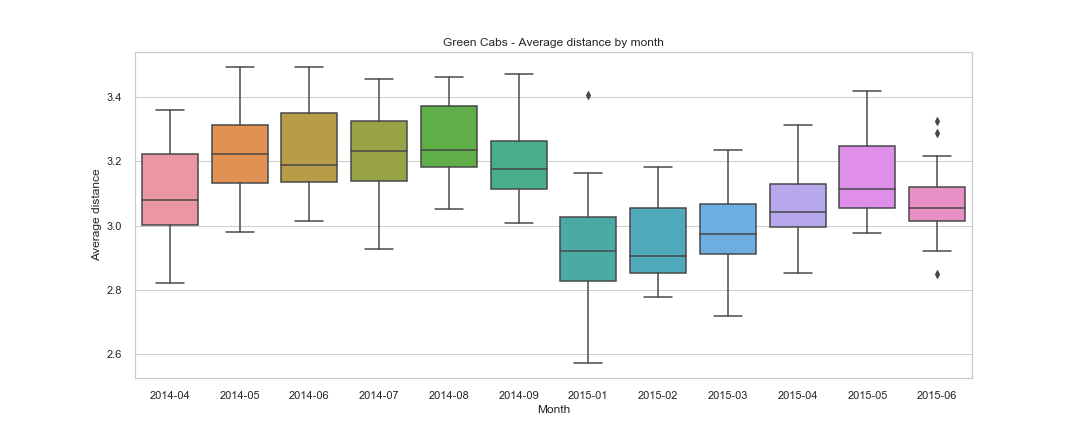
\includegraphics[height=2in, width=3.5in]{green_avgdistance_month.png}}%
\caption{Distance analysis for Yellow and Green cabs. Images a and c shows the monthly average price per distance. Images b and d show the average distance per month.}
\label{fig:boxDistancesPrice}%
\end{figure}






\subsubsection{Heat Maps}
\label{secc:heatMaps}
In this section different maps were created to analyze which areas of the city, in terms of NTAs, are the ones with less coverage; or what are the most common transportation choices of people, per NTA. Two different maps were created. The first one, Figure \ref{fig:heatMapTripsPick}, shows the number of pick-ups and and the pickup zone, of the different transportation options. On the other hand, Figure \ref{fig:heatMapTripsDrop}, shows the number of drop-offs and the drop-off zones.

Table \ref{tab:dataset} shows the Links to access the interactive Heat Maps. The maps show the number of trips per NTA, in the different transportation options.

\begin{table}[h]
\begin{center}
\begin{tabular}{|c|c|}
\hline
\textbf{Figure Name}     & \textbf{Link to Map}  \\ 
\hline
Trips NTA Green Dropoff Map     & \href{https://marioceron-case-51.s3.amazonaws.com/datathon_html/trips_nta_green_dropoff_map.html}{Link}   \\
Trips NTA MTA Dropoff Map       & \href{https://marioceron-case-51.s3.amazonaws.com/datathon_html/trips_nta_mta_dropoff_map.html}{Link}   \\
Trips NTA Yellow Dropoff Map    & \href{https://marioceron-case-51.s3.amazonaws.com/datathon_html/trips_nta_yellow_dropoff_map.html}{Link}  \\
Trips Population NTA Green Map  & \href{https://marioceron-case-51.s3.amazonaws.com/datathon_html/trips_pop_nta_green_map.html}{Link}      \\
Trips Population NTA MTA Map    & \href{https://marioceron-case-51.s3.amazonaws.com/datathon_html/trips_pop_nta_mta_map.html}{Link}       \\
Trips Population NTA Uber Map  & \href{https://marioceron-case-51.s3.amazonaws.com/datathon_html/trips_pop_nta_uber_map.html}{Link}      \\
Trips Population NTA Yellow Map & \href{https://marioceron-case-51.s3.amazonaws.com/datathon_html/trips_pop_nta_yellow_map.html}{Link}\\

Total Pick Ups per NTA & \href{https://marioceron-case-51.s3.amazonaws.com/datathon_html/trips_nta_total_pickup.html}{Link}\\
Total Drop Offs & \href{https://marioceron-case-51.s3.amazonaws.com/datathon_html/trips_nta_max_coverage_dropoff.html}{Link}\\
Pick Ups & \href{https://marioceron-case-51.s3.amazonaws.com/datathon_html/trips_nta_max_coverage.html}{Link}\\
Drop Offs & \href{https://marioceron-case-51.s3.amazonaws.com/datathon_html/trips_nta_max_coverage_dropoff.html}{Link}\\
 \hline
\end{tabular}
 \caption{Links to access interactive Heat Maps. The maps show the number of trips per NTA, in the different transportation options.}
 \label{tab:dataset}
\end{center}
\end{table}



\begin{figure}%
\centering
\subfigure[Uber.]{%
\label{fig:a}%
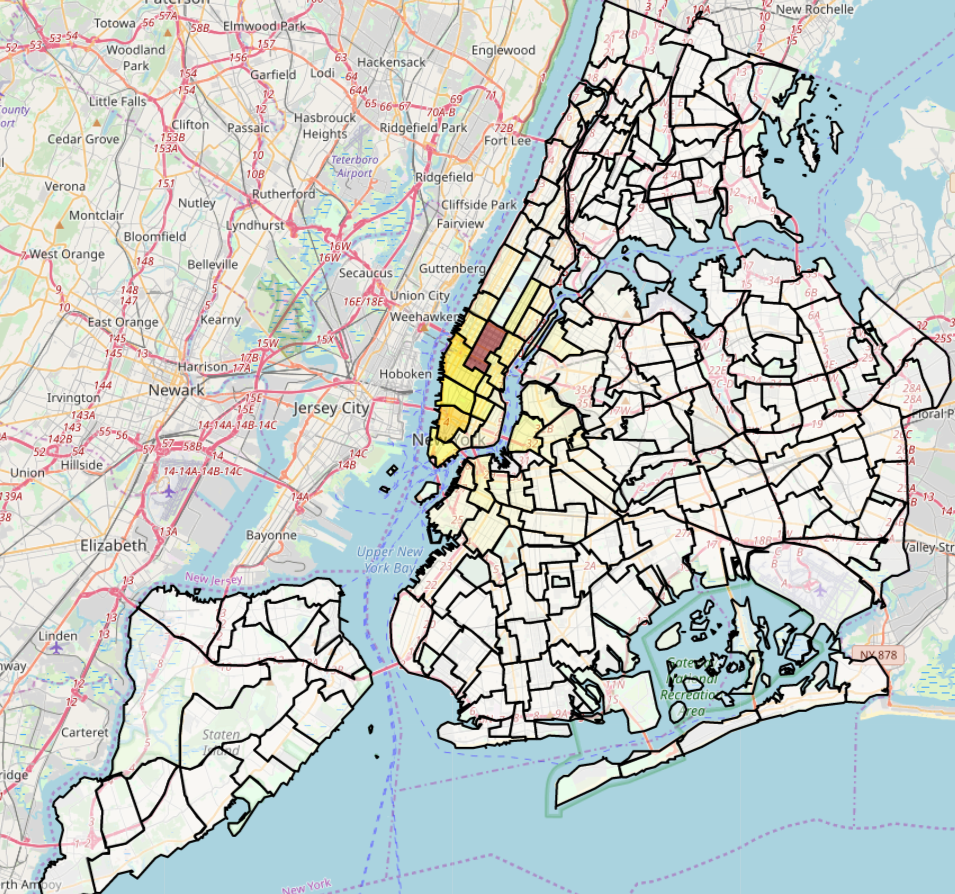
\includegraphics[height=2.5in, width=3in]{uberNormPopulation_pickup.png}}%
\subfigure[Yellow cab]{%
\label{fig:b}%
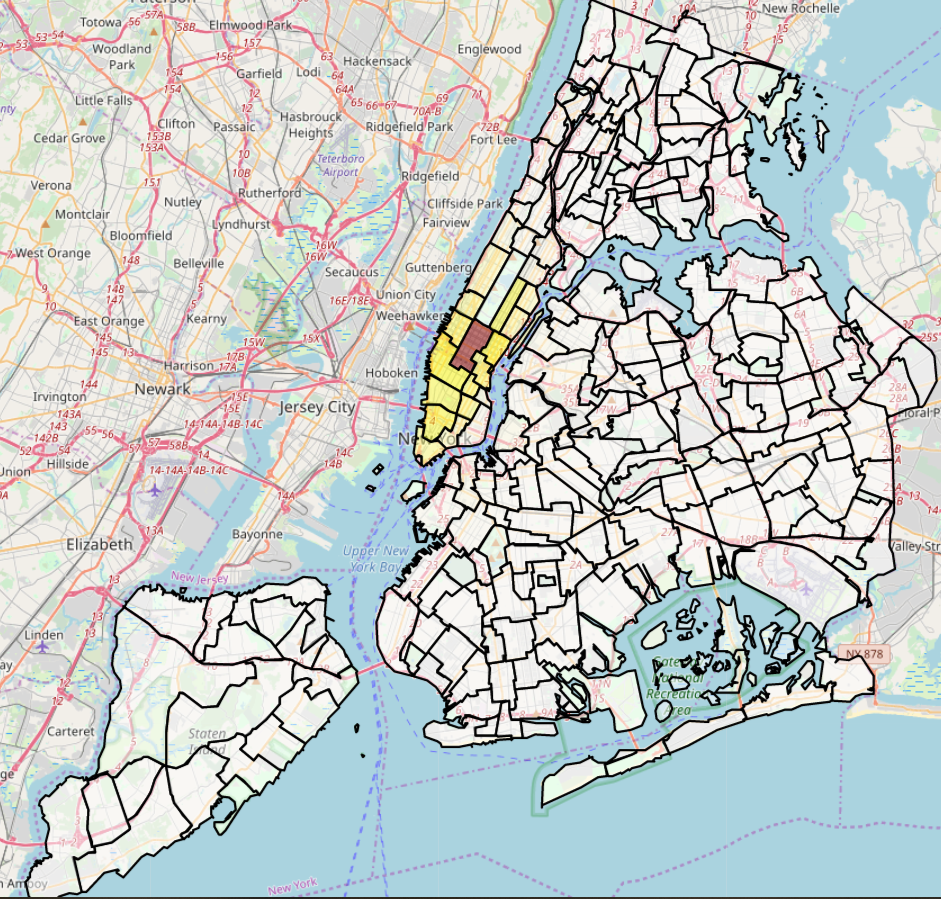
\includegraphics[height=2.5in, width=3in]{yellowNormPopulation_pickup.png}}
\qquad
\subfigure[Green cab ]{%
\label{fig:c}%
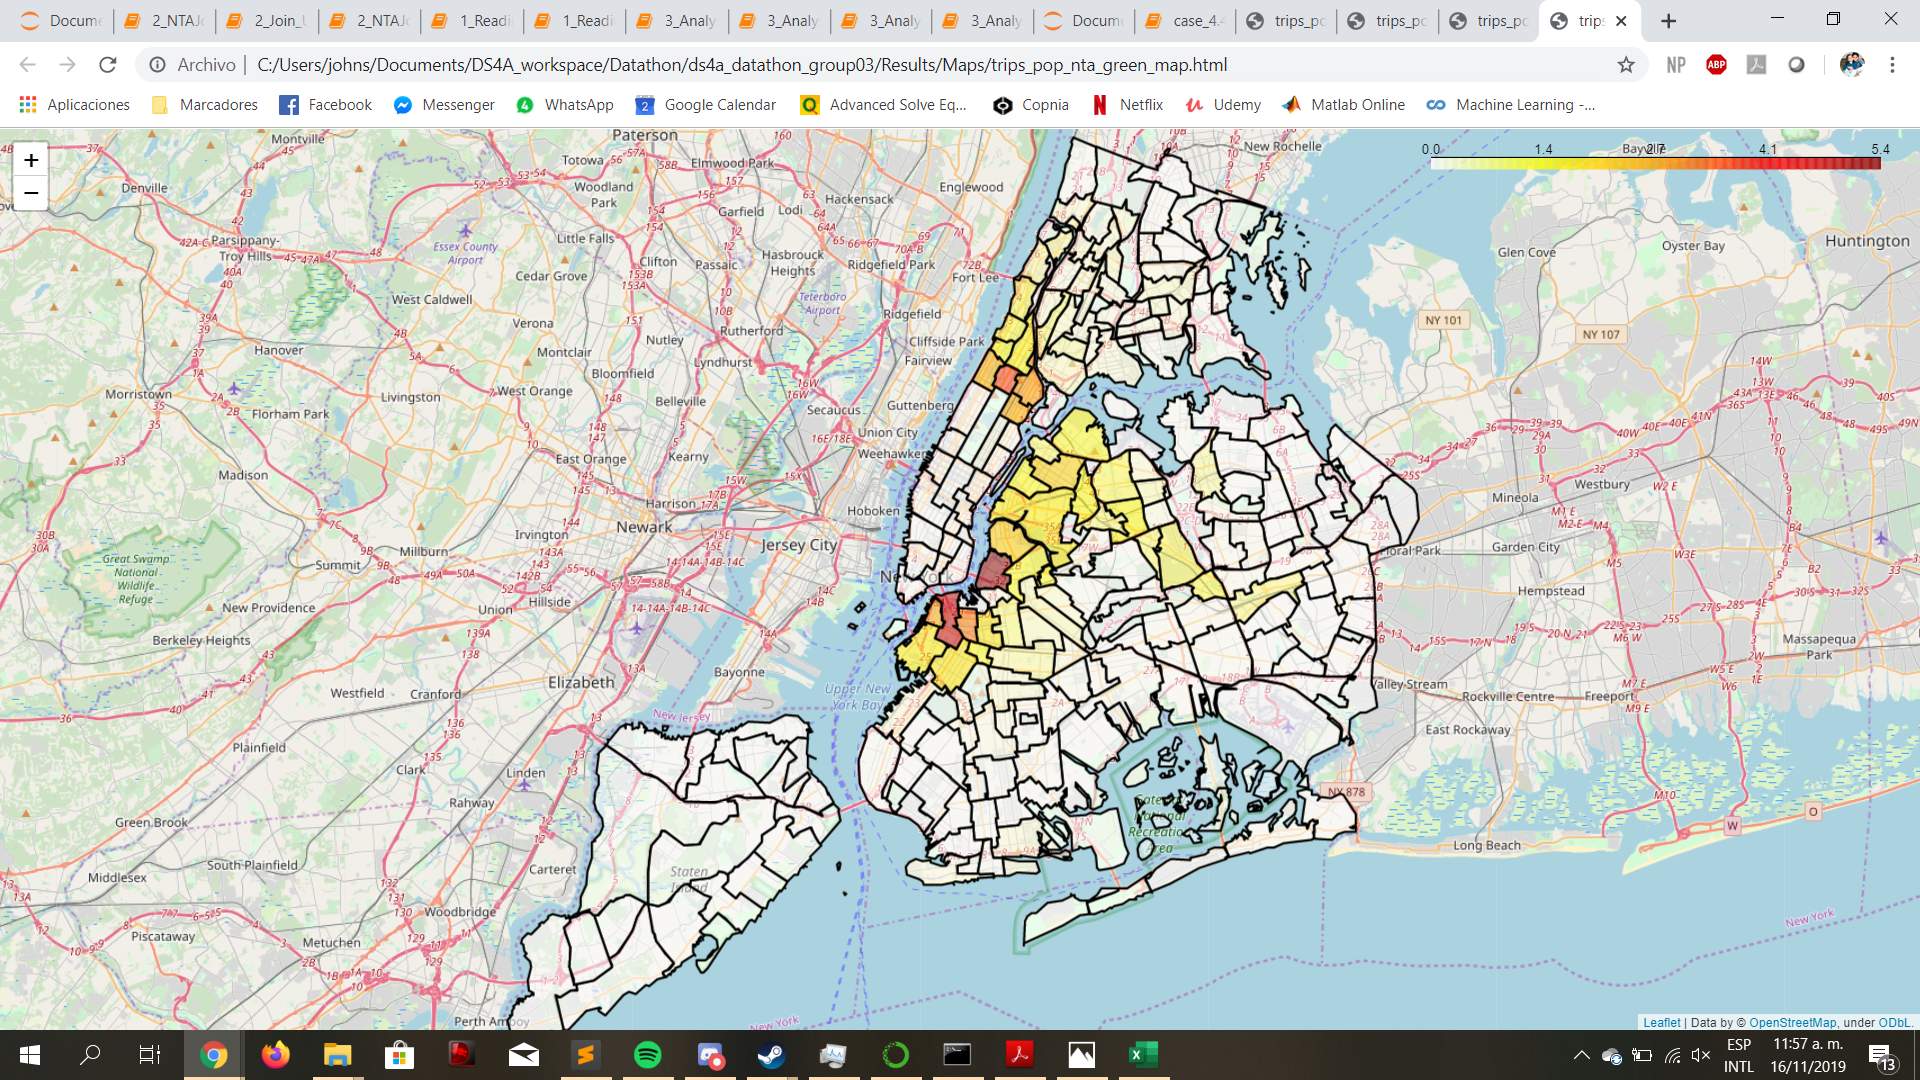
\includegraphics[height=2.5in, width=3in] {greenNormPopulation_pickup.png}}
\subfigure[MTA ]{%
\label{fig:d}%
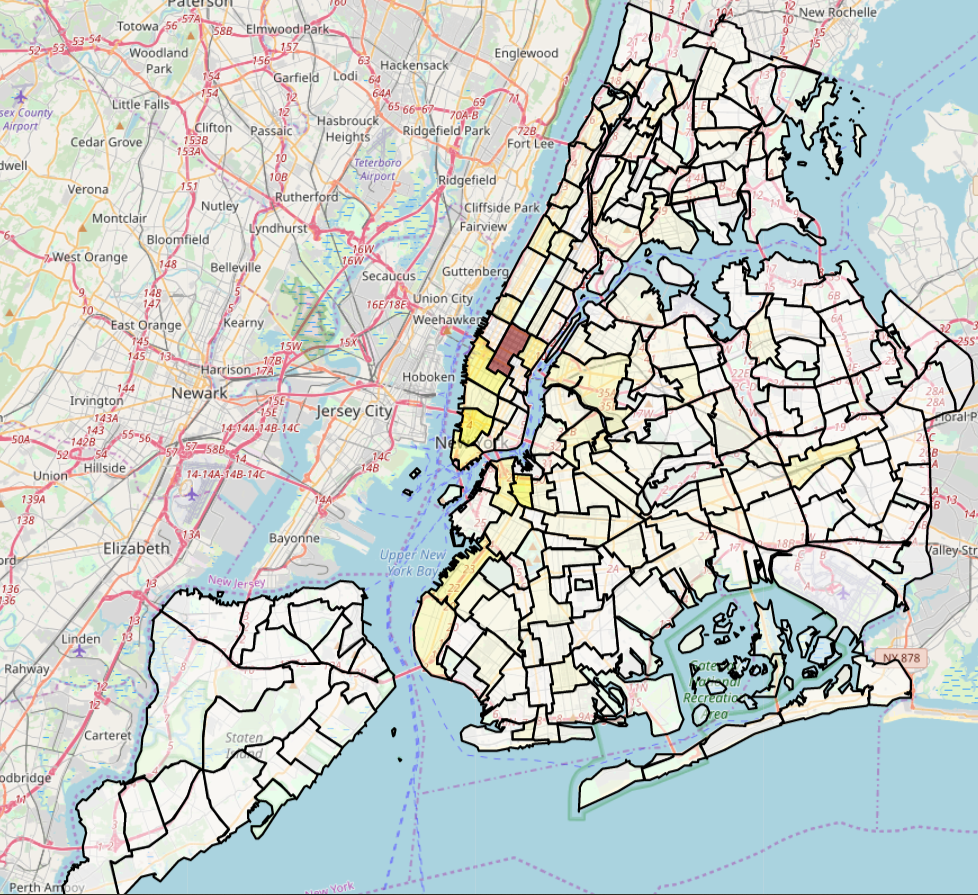
\includegraphics[height=2.5in, width=3in] {mtaNormPopulation_pickup.png}
}%
\caption{Heat maps of Pick Ups. The maps show the number of trips per NTA, in the different transportation options. The data has been normalized by the NTA population.}
\label{fig:heatMapTripsPick}%
\end{figure}


\begin{figure}%
\centering
\subfigure[Yellow cab trips]{%
\label{fig:b}%
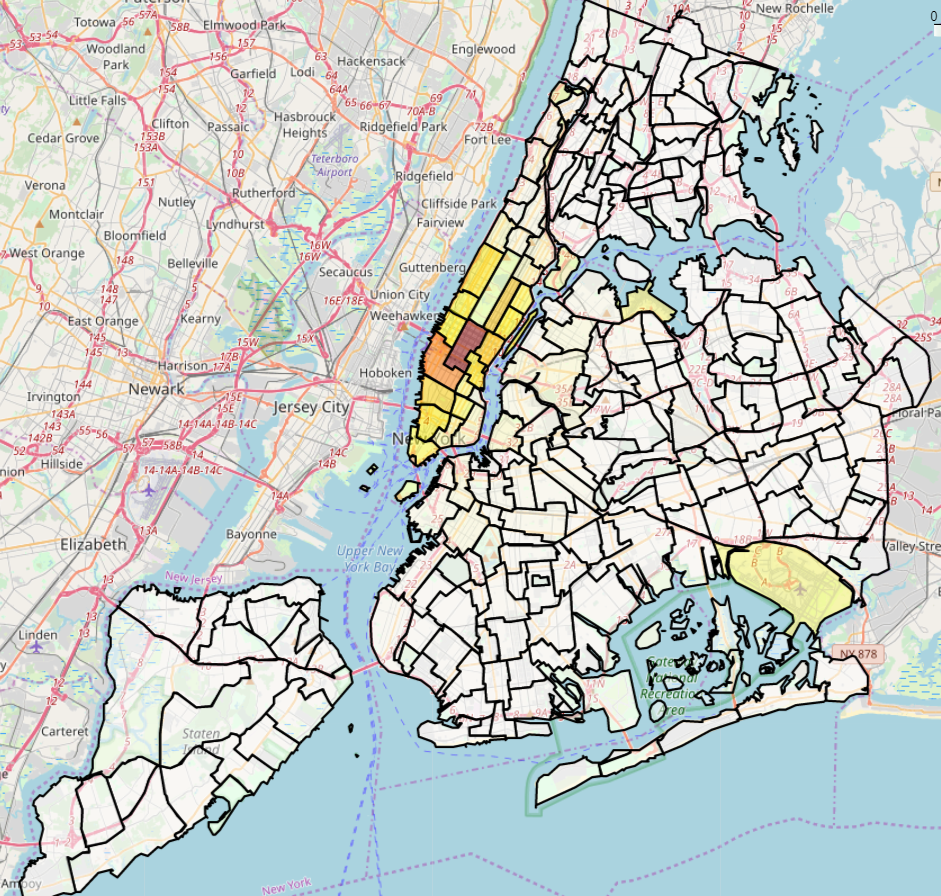
\includegraphics[height=2.5in, width=3in]{yellowNormPopulation_dropoff.png}}
\qquad
\subfigure[Green cab trips]{%
\label{fig:c}%
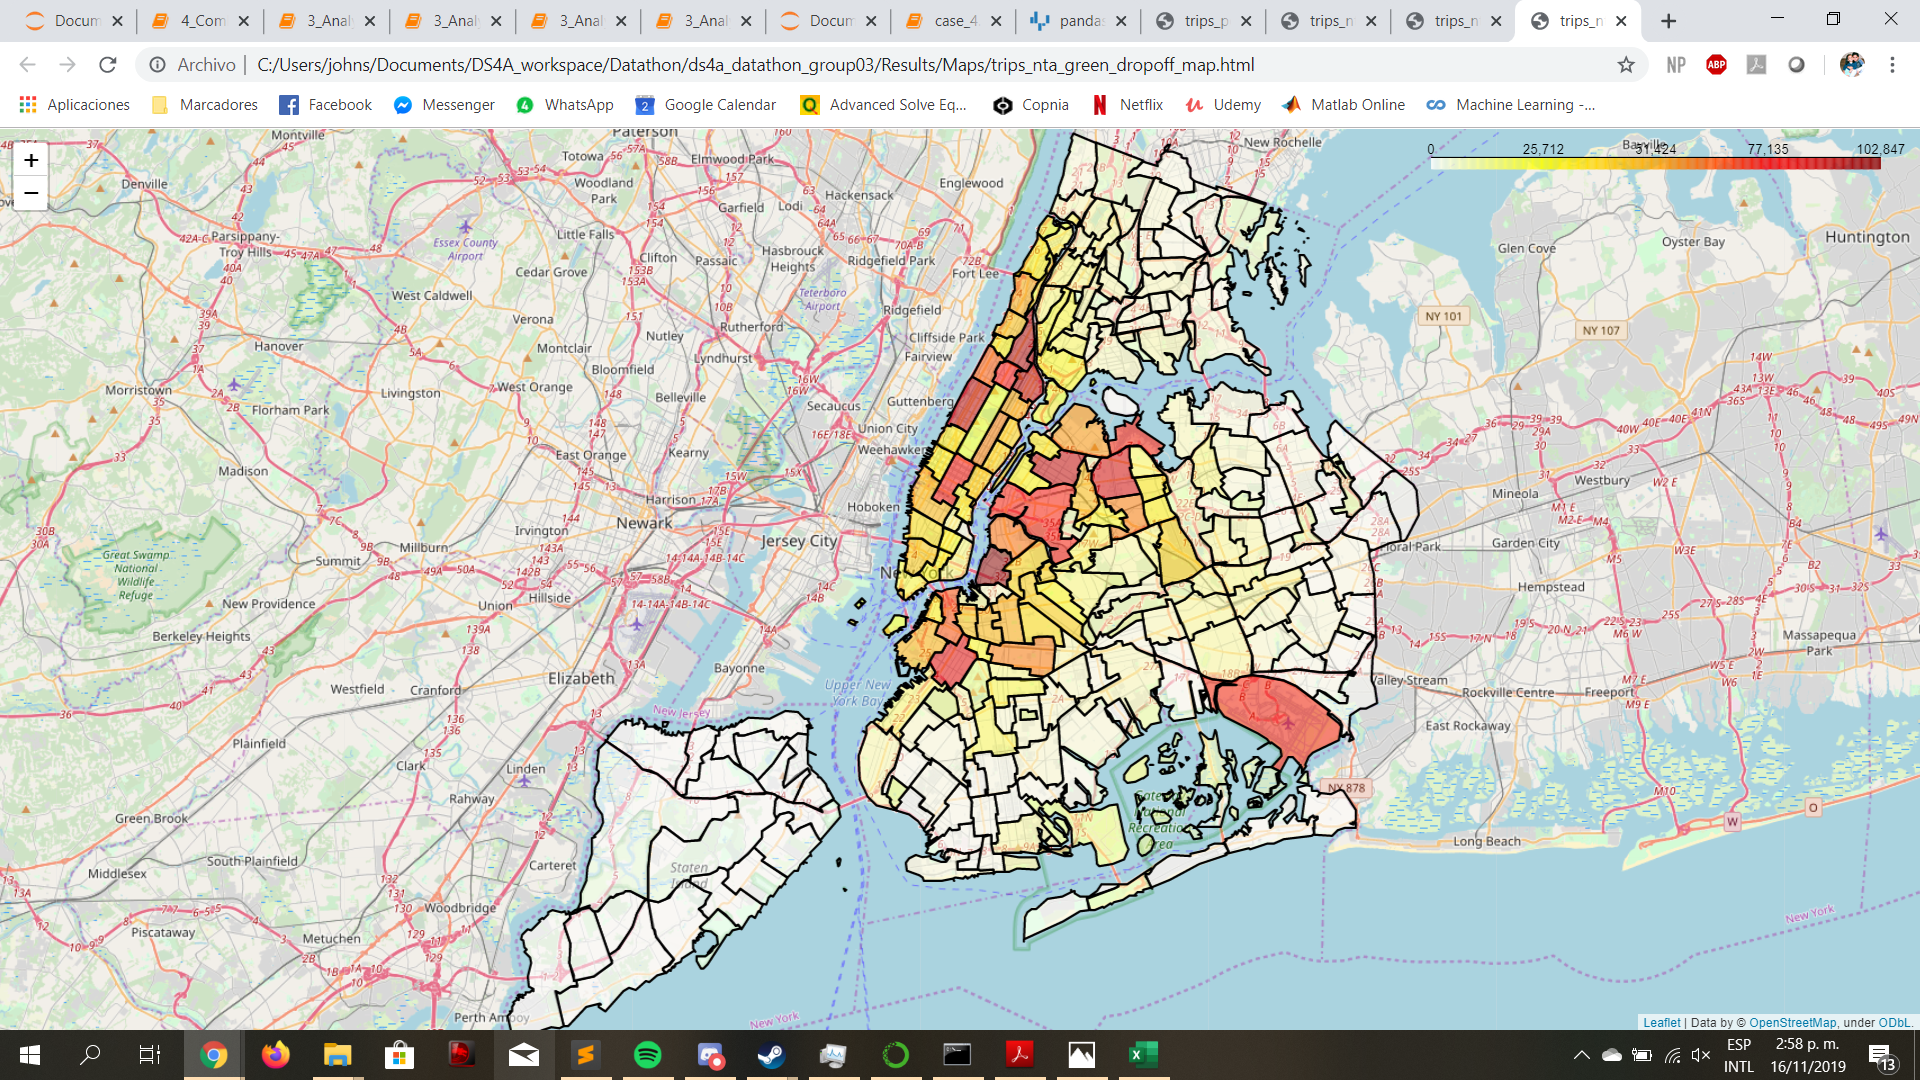
\includegraphics[height=2.5in, width=3in] {greenNormPopulation_dropoff.png}}
\subfigure[MTA trips]{%
\label{fig:d}%
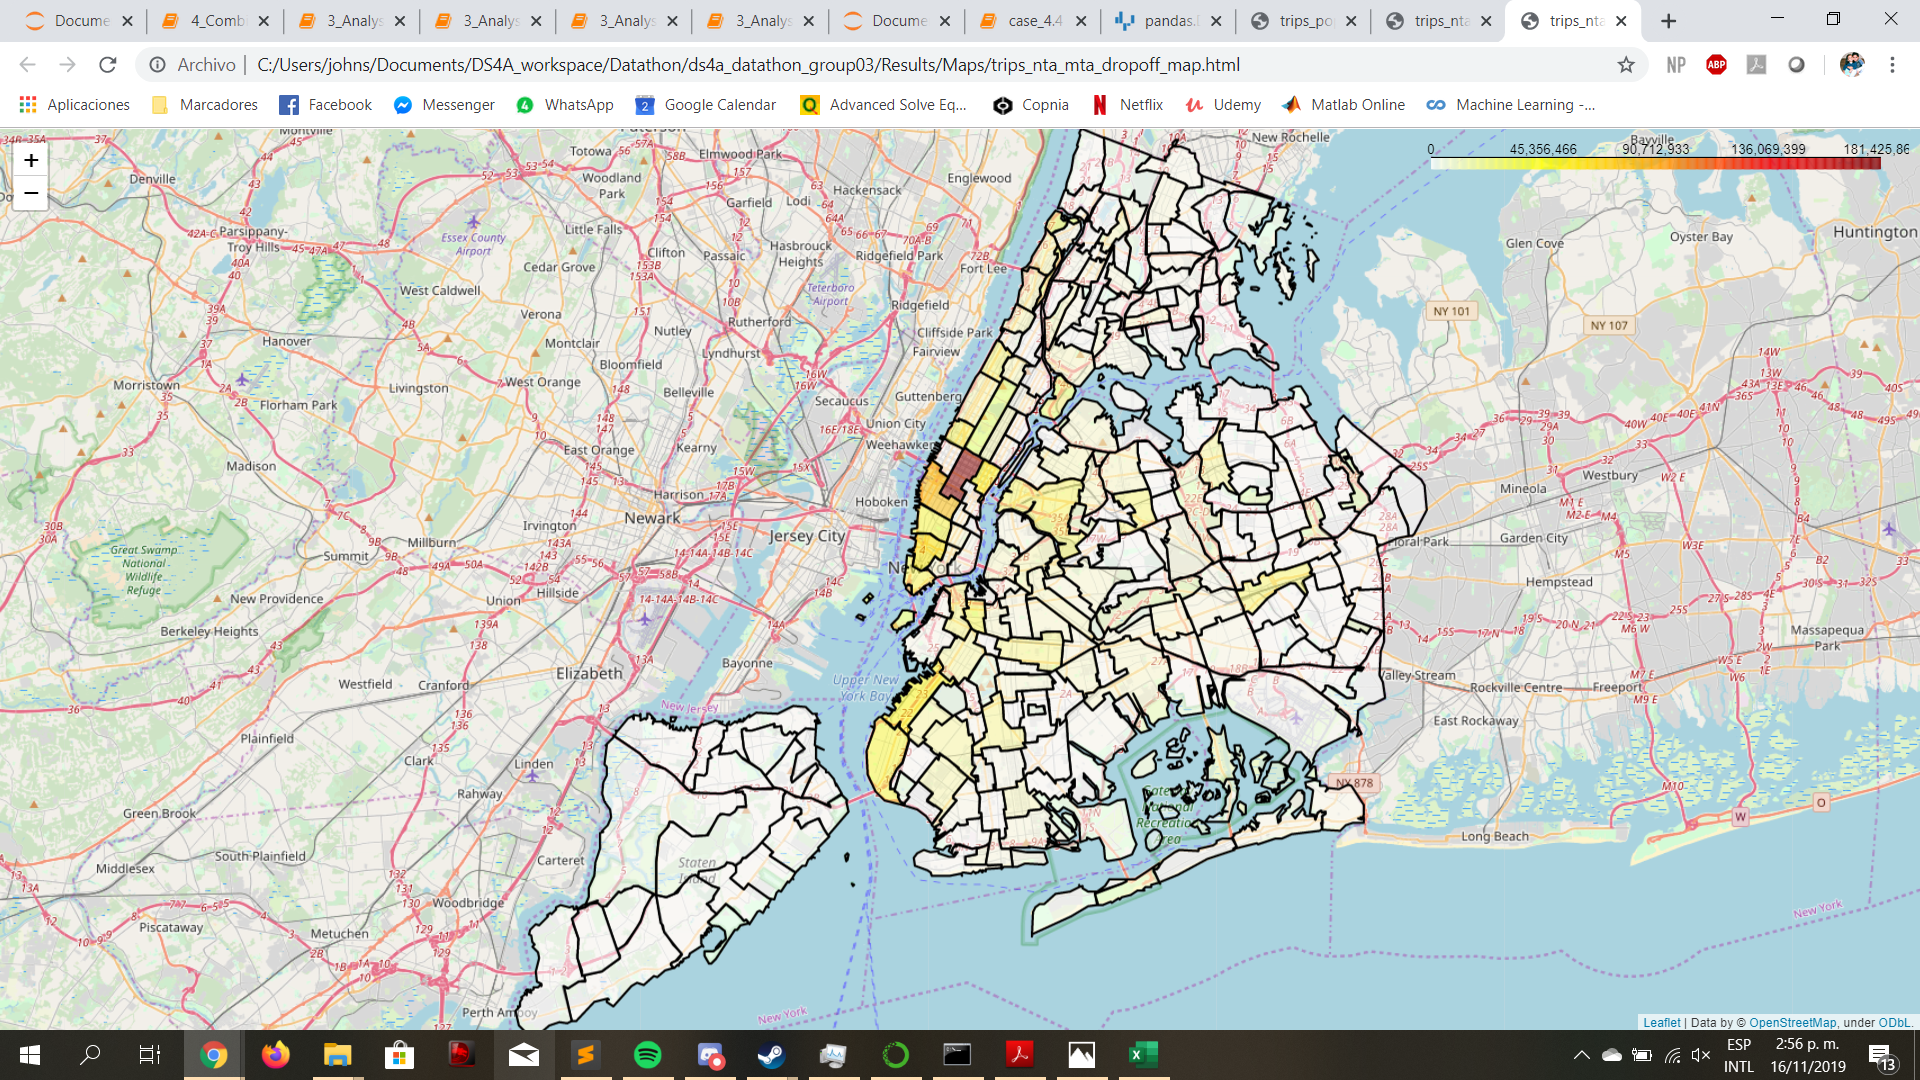
\includegraphics[height=2.5in, width=3in] {mtaNormPopulation_dropoff.png}
}%
\caption{Heat maps of Drop offs. The maps show the number of trips per NTA, in the different transportation options. }
\label{fig:heatMapTripsDrop}%
\end{figure}





Figure \ref{fig:heatMapTotalPickDrop} shows the location and the total number of pick ups and drop offs, of Green, Yellow, UBER (only pick up information was available) and MTA transportation means. The data is normalized by the population of each MTA. These maps start showing areas where public transportation is not widely used.


\begin{figure}%
\centering
\subfigure[Total Pick Ups per NTA]{%
\label{fig:heatMapTotalPickDrop_a}%
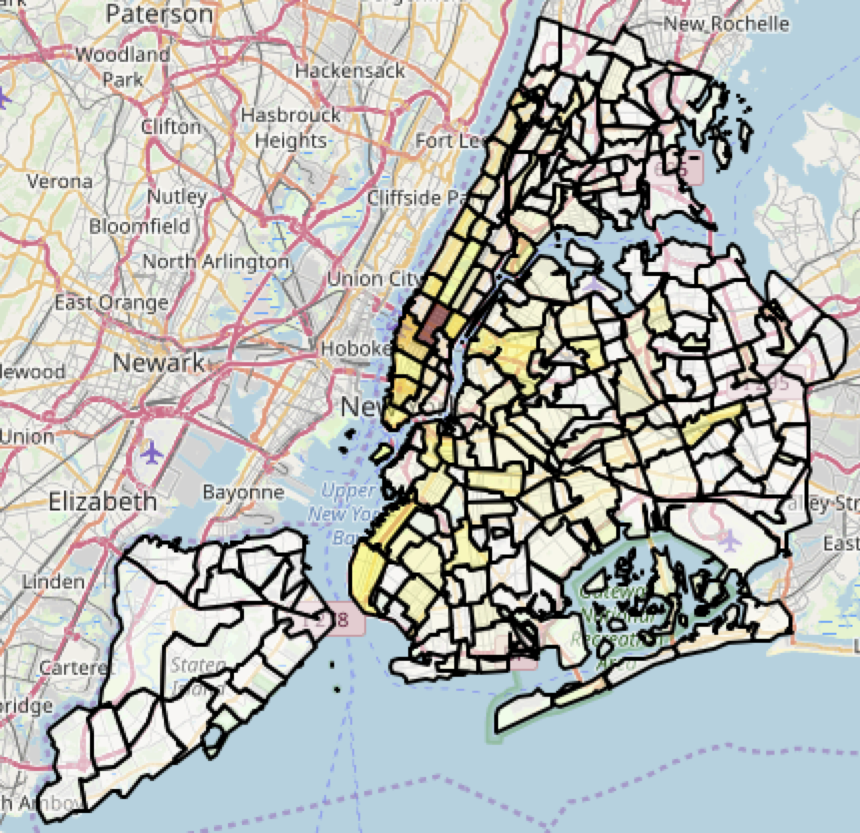
\includegraphics[height=2.5in, width=3in]{totalNormPickUps.png}}
\qquad
\subfigure[Total Drop Offs]{%
\label{fig:heatMapTotalPickDrop_b}%
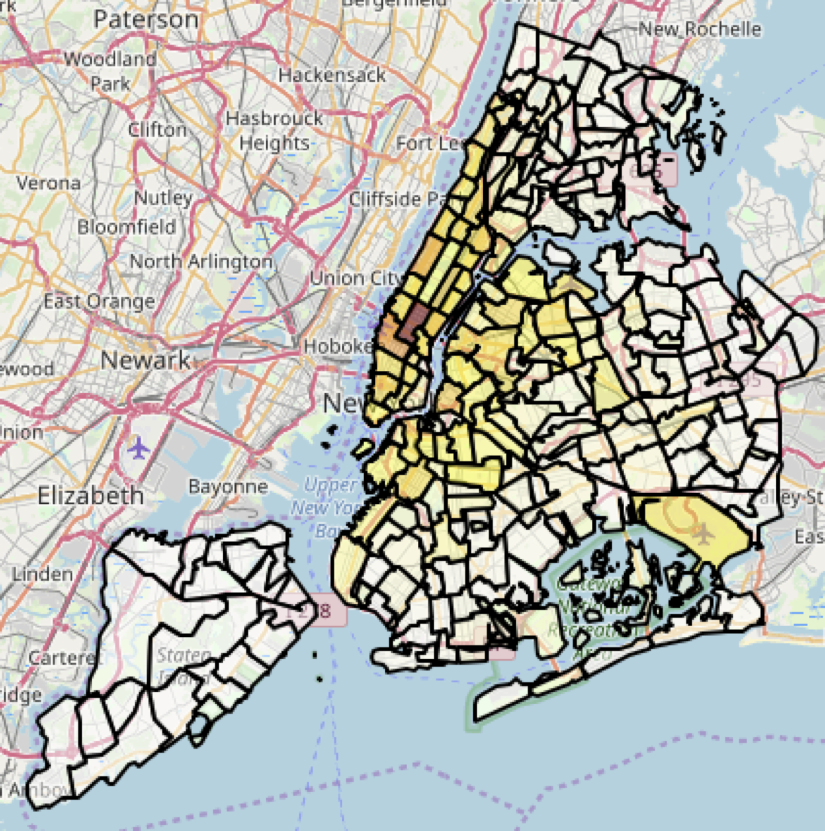
\includegraphics[height=2.5in, width=3in] {totalNormDropOffs.png}}
\caption{Analyzing the total number of Pick Ups and Drop Off of all the transportation options. }
\label{fig:heatMapTotalPickDrop}%
\end{figure}



On the other hand, Figure \ref{fig:maxMapTotalPickDrop} shows per NTA, which is the transportation option more used in the area. Analyzing the map that appears on the left (Pick ups), it can be seen that in the outer areas of the city, UBER is widely used. However, MTA is the prefer transportation option in most of the city. The latter coincides with what was found in Section \ref{intro_background}: NYC is famous because people does not like to own a car, they prefer to use public transportation.

The right figure shows the drop off map. It is important to remember that there is no drop off information of UBER, and this is why in the outer areas, it is possible see that yellow and green cabs options are widely used. This map is different from what we expected. The reason is that according to the literature, Yellow cars do not like to move far from Manhattan. However, the map shows that they are moving far from it.


\begin{figure}%
\centering
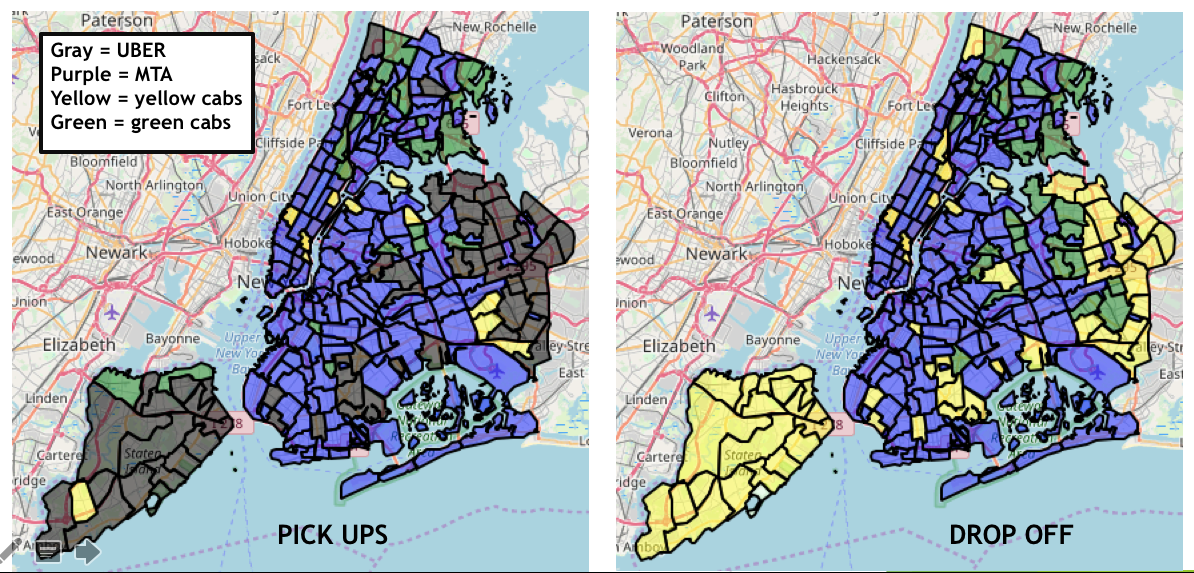
\includegraphics[height=3.5in, width=7in]{maxOptionMap.png}
\caption{Most frequently transportation mean per NTA. The maps show the number of trips per NTA, in the different transportation options.}
\label{fig:maxMapTotalPickDrop}%
\end{figure}

